\documentclass[english,11pt]{beamer}

\DeclareMathOperator{\Cov}{Cov}
\DeclareMathOperator{\Var}{Var}
\DeclareMathOperator{\E}{\mathbb{E}}
\DeclareMathOperator{\Proba}{\mathbb{P}}

\newcommand{\Covb}[2]{\ensuremath{\Cov\!\left[#1,#2\right]}}
\newcommand{\Eb}[1]{\ensuremath{\E\!\left[#1\right]}}
\newcommand{\Pb}[1]{\ensuremath{\Proba\!\left[#1\right]}}
\newcommand{\Varb}[1]{\ensuremath{\Var\!\left[#1\right]}}

% norm
\newcommand{\norm}[1]{\| #1 \|}

\newcommand{\indep}{\rotatebox[origin=c]{90}{$\models$}}





\usepackage{mathptmx,amsmath,amssymb,graphicx,bibentry,bbm,babel,ragged2e}

\makeatletter

\newcommand{\noun}[1]{\textsc{#1}}
\newcommand{\jitem}[1]{\item \begin{justify} #1 \end{justify} \vfill{}}
\newcommand{\sframe}[2]{\frame{\frametitle{#1} #2}}

\newenvironment{centercolumns}{\begin{columns}[c]}{\end{columns}}
%\newenvironment{jitem}{\begin{justify}\begin{itemize}}{\end{itemize}\end{justify}}

\usetheme{Warsaw}
\setbeamertemplate{footline}[text line]{}
\setbeamercolor{structure}{fg=purple!50!blue, bg=purple!50!blue}

\setbeamersize{text margin left=15pt,text margin right=15pt}

\setbeamercovered{transparent}


\@ifundefined{showcaptionsetup}{}{%
 \PassOptionsToPackage{caption=false}{subfig}}
\usepackage{subfig}

\usepackage[utf8]{inputenc}
\usepackage[T1]{fontenc}



\makeatother

\begin{document}


\title{Modeling the Co-evolution of Urban Form and Transportation Networks}

\author{J.~Raimbault$^{1,2,\ast}$\\
\texttt{juste.raimbault@polytechnique.edu}
}


\institute{$^{1}$UMR CNRS 8504 G{\'e}ographie-cit{\'e}s\\
$^{2}$UMR-T IFSTTAR 9403 LVMT
}


\date{Sageo 2017 - Rouen\\\smallskip
November 7th 2017
}

\frame{\maketitle}





%%%%%%%%%%%%%%%%%%%
%% ABSTRACT

%\keywords{Spatio-temporal Causality ; Network-territories Interactions ; Urban Morphogenesis ; Greater Paris}
%This paper contributes to the understanding of strongly coupled spatio-temporal processes by describing a generic method based on Granger causality. The method is validated by the robust identification of causality regimes and of their phase diagram for an urban morphogenesis model that couples network growth with density. The application to the real case study of Greater Paris transportation projects shows a link between territorial dynamics, more particularly of real estate and socio-economic, and the anticipated network growth. We finally discuss potential extensions to other temporal and spatial scales.



%%%%%%%%%%%%%%%%%
\section{Introduction}
%%%%%%%%%%%%%%%%%



\sframe{Circular Causalities in Complex Systems}{

\centering

% striking image

%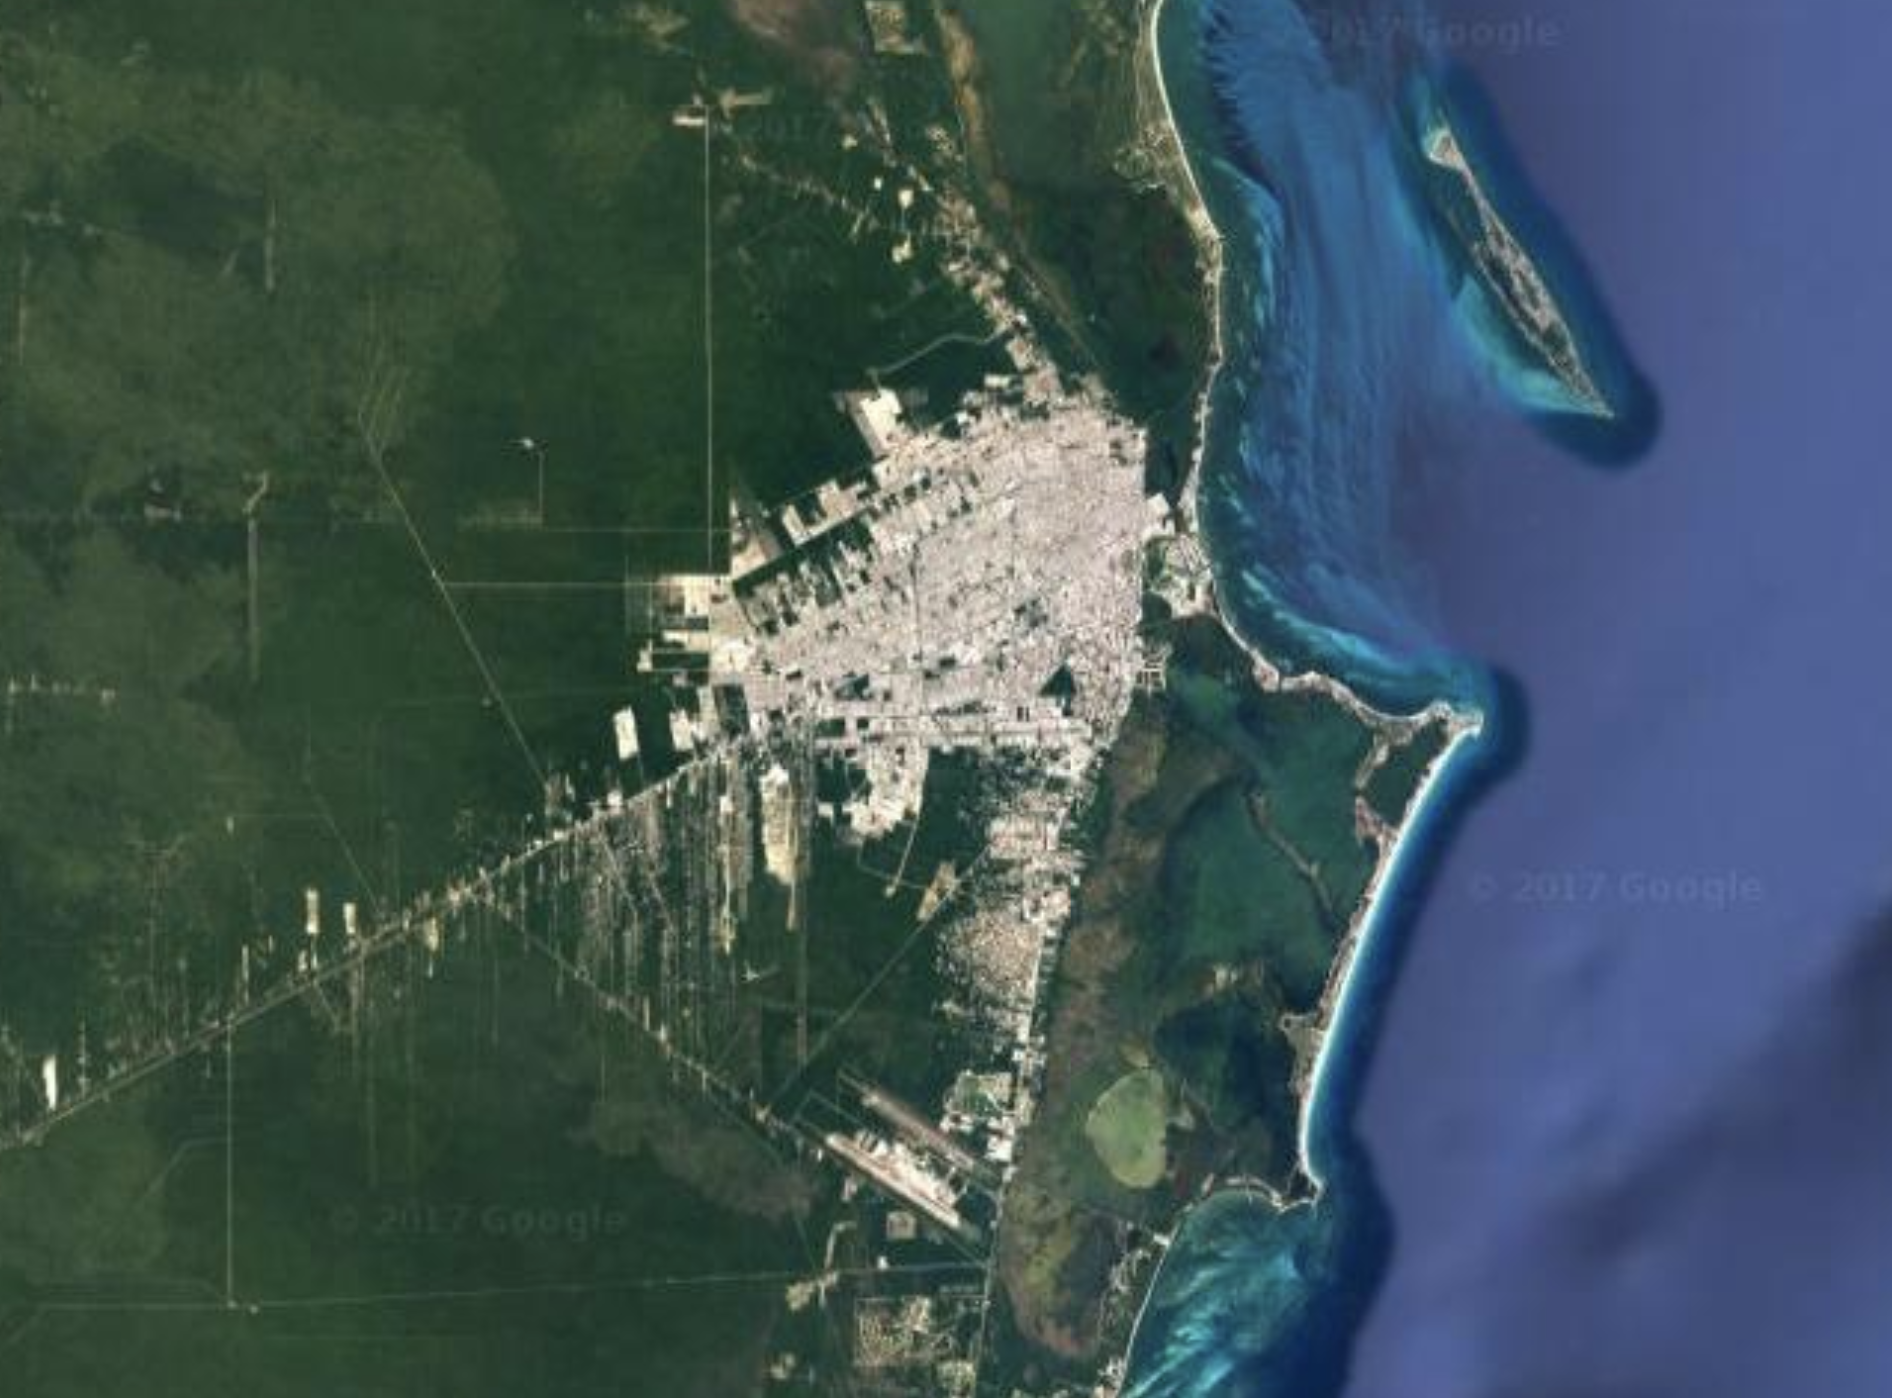
\includegraphics[width=0.8\textwidth]{figures/cancun}

\footnotesize\textit{Source: }

}


\sframe{Causality in Geography}{


}

\sframe{Existing approaches}{


}

\sframe{Research objective}{


}





%%%%%%%%%%%%%%%%%
\section{Methods and Results}
%%%%%%%%%%%%%%%%%


\sframe{Method: Rationale}{

}


\sframe{Method: Formalization}{

}

\sframe{Validation: Synthetic Data}{

% present strategy and rbd model

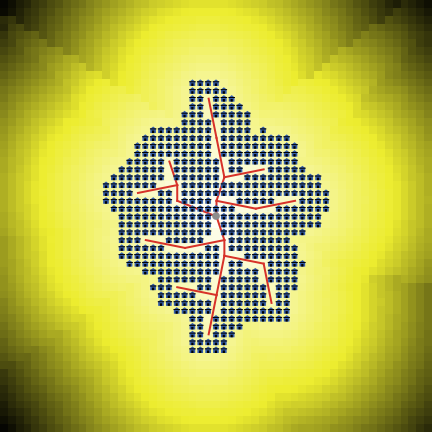
\includegraphics[width=0.32\textwidth]{figures/ex_60_wdens0_wroad1_wcenter1_seed272727}
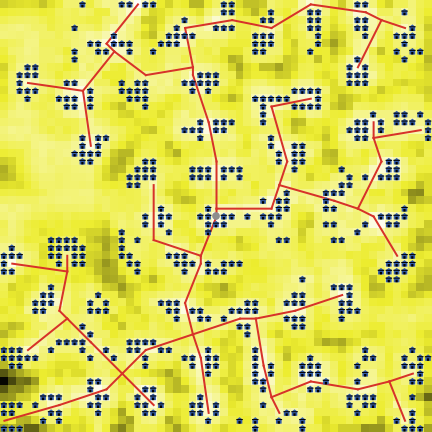
\includegraphics[width=0.32\textwidth]{figures/ex_60_wdens1_wroad1_wcenter0_seed272727}
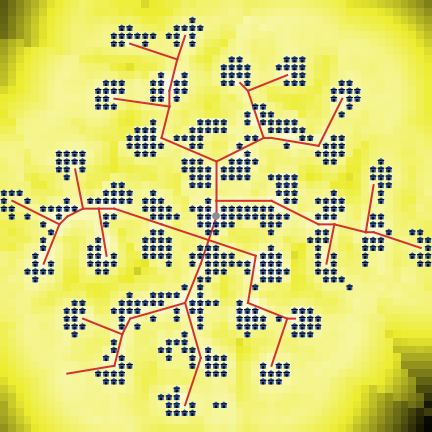
\includegraphics[width=0.32]{figures/ex_60_wdens1_wroad1_wcenter1_seed272727}

}


\sframe{Endogenous causality regimes}{

}


\sframe{Application: Case study}{

}


\sframe{Application: Results}{

}



%%%%%%%%%%%%%%%%%
\section{Discussion}
%%%%%%%%%%%%%%%%%





\sframe{Discussion}{

\justify

\vspace{-1cm}

\textbf{Implications}

$\rightarrow$ 

\bigskip

\textbf{Developments}


$\rightarrow$ 

}




\sframe{Conclusion}{

\justify

$\rightarrow$ 

\bigskip
\bigskip
\bigskip

\footnotesize{ - Code, data and results available at\\ \texttt{https://github.com/JusteRaimbault/CityNetwork}

}

}






\sframe{Reserve slides}{

\centering

\Large

\textbf{Reserve Slides}

}




%%%%%%%%%%%%%%%%%%%%%
\begin{frame}[allowframebreaks]
\frametitle{References}
\bibliographystyle{apalike}
\bibliography{/Users/juste/ComplexSystems/CityNetwork/Biblio/Bibtex/CityNetwork,biblio}
\end{frame}
%%%%%%%%%%%%%%%%%%%%%%%%%%%%









\end{document}







